\documentclass[../main.tex]{subfiles}

\begin{document}

\problem{2}


\assumptions{}
Inviscid, isentropic flow outside the shocks.
Flat plates are infinitesimally thin and do not disturb the flow.
All figures are extremely qualitative.
Static pressures return to approximately atmospheric conditions after the bodies. 

\begin{itemize}

    \item Flat plate with no incidence: Figures \ref{flat_shock}-\ref{flat_pressure} qualitatively show the flow over a flat plate in supersonic flow with no incidence angle.
    Because the supersonic flow is not turned (assuming inviscid flow), there is no dissipative shock generated.
    Instead, weak Mach waves emanate from the leading edge of the plate.
    The static pressure is constant with Mach number (assuming freestream static pressure is identical for all Mach numbers shown).
    When put at an incidence angle to the flow, an expansion wave is generated on the top surface, and an oblique shock on the bottom.
    The pressure on top is reduced, and the pressure on bottom is increased accordingly.
    The flow on the top and bottom surfaces go through the opposite process at the trailing edge in order to return to approximately atmospheric pressure. 

    \item Flat plate with incidence: Figures \ref{incidence_shock}-\ref{incidence_pressure} qualitatively show the flow over a flat plate in supersonic flow with an incidence angle.
    On the top surface an expansion wave is generated while on the bottom surface an oblique shock is formed.
    Pressure is reduced on top and increased on bottom. 
    For greater Mach numbers, the expansion wave on top is stronger and accelerates flow/reduces pressure more than the baseline case.
    Similarly, the oblique shock on the bottom surface is stronger for a larger freestream Mach number and generates a larger static pressure after the shock compared to the baseline case.
    If the incidence angle is increased, the expansion wave and oblique shock both grow stronger, similar to the increased Mach case, although the exact quantity of increase depends on geometry and flow specifics.
    The larger incidence angle causes stronger flow features because the flow must turn a greater amount.
    At the trailing edge the flow on top and bottom undergo the opposite process as the leading edge in order to return to approximately atmospheric conditions. 

    \item Diamond wedge: Figures \ref{diamond_shock}-\ref{diamond_pressure} qualitatively show the flow over a diamond wedge with no incidence.
    The flow over this body is symmetrical on the top and bottom surfaces.
    At the leading edge an oblique shock forms due to the turning angle of the wedge, causing a pressure rise.
    At the apex of the wedge, an expansion wave turns the flow back in the direction of the aft surfaces, reducing pressure.
    The flow at the trailing edge experiences an oblique shock due to the impingement of the angled top/bottom flows, restoring them to atmospheric pressure and turning them back horizontal.
    For a larger Mach number the same behavior is observed with increased oblique shock and expansion wave strength.
    Both higher and lower static pressure values are observed for a larger Mach number.
    The expansion wave is stronger because the local Mach number after the oblique shock for the higher freestream Mach case will be larger than the baseline case, allowing the flow to accelerate more with a similarly increased pressure drop.
    When the wedge is at an angle of incidence, the shock on the top surface is weakened, causing a lower pressure, while the shock on the bottom is strengthened, causing a higher pressure.
    The expansion wave on the top surface is stronger than the one on the bottom because of the larger Mach number.
    The pressure after the expansion on top is lower than the baseline case whereas the bottom pressure is higher than the baseline case.
    
    \item Biconvex: Figures \ref{bi_shock}-\ref{bi_pressure} qualitatively show the flow over a biconvex airfoil with no incidence.
    There is an attached oblique shock at the leading edge causing a static pressure rise. 
    This shock becomes weaker over time, and the geometry of the biconvex airfoil turns away from the flow, generating an expansion region, reducing the pressure.
    Another expansion region forms after the midpoint of the airfoil when the surface again turns away, further reducing the pressure.
    Finally, an oblique shock is generated at the trailing edge where the two supersonic flows impinge upon each other, straightening them and restoring them to approximately atmospheric pressure.
    For a larger Mach number, stronger oblique shocks and expansion waves are observed, with commensurate increases in pressure extremes.
    If the airfoil were at an angle of incidence, the shock on the top surface is weakened, but the expansions are strengthed.
    The opposite behavior is observed on the bottom surface due to the increased turning angle.
    
    \item Diamond block: Figures \ref{block_shock}-\ref{block_pressure} qualitatively show the flow over a diamond block with no incidence.
    Similar to the diamond wedge, an oblique shock is attached to the leading edge followed by an expansion fan when the geometry turns horizontally.
    The major difference occurs at the aft end, where there is a base area at a right angle to the top and bottom surfaces.
    The flow cannot fully turn perpendicularly but does experience an expansion fan with a reduction in pressure over the back end.
    There is a complex region immediately behind the base before the top and bottom streamlines impinge and shock back to atmospheric pressure.
    The details of the flow in this region are complex and beyond the quasi-1-D isentropic flow regime that we have been analyzing.
    For larger Mach numbers, the shock and expansion wave strength are increased as in previous cases.
    If the geometry were put at an angle of incidence to the flow, the oblique shock on the top is weakened while the one on the bottom is strengthened, with the opposite occurring for the expansion waves.

    \item If pressures were measured while standing on the ground (ignoring any potential shock interactions), the plots would not change.
    This assumes that we are close enough to the body that the air has not mixed with stagnant air and returned to atmospheric conditions (ignoring dissipative effects from a distance).
    Near the body, flow can be approximated as isentropic and constant in the regions between shocks and expansions.
    Because we have explicitly ignored viscous effects, we assume that the flow properties at the wall and off the body are the same.
    In real life, flow properties on the wall would be very different than those at a distance due to the viscous boundary layer and the no-slip condition. 

    \item \textbf{Assuming invviscid flow:} The flate plate at no incidence would not generate lift nor drag because it has no impact on the flow.
    The other geometries would all generate drag due to the differential pressure caused by the shock-expansion processes on the body.
    Only the flate plate at an angle of incidence would generate lift due to the asymmetric distribution of pressure on the top and bottom surfaces.
    The other geometries do not experience a net pressure force in the \(y\)-direction. 

\end{itemize}

\newpage

\begin{figure}[h!]
    \centering
    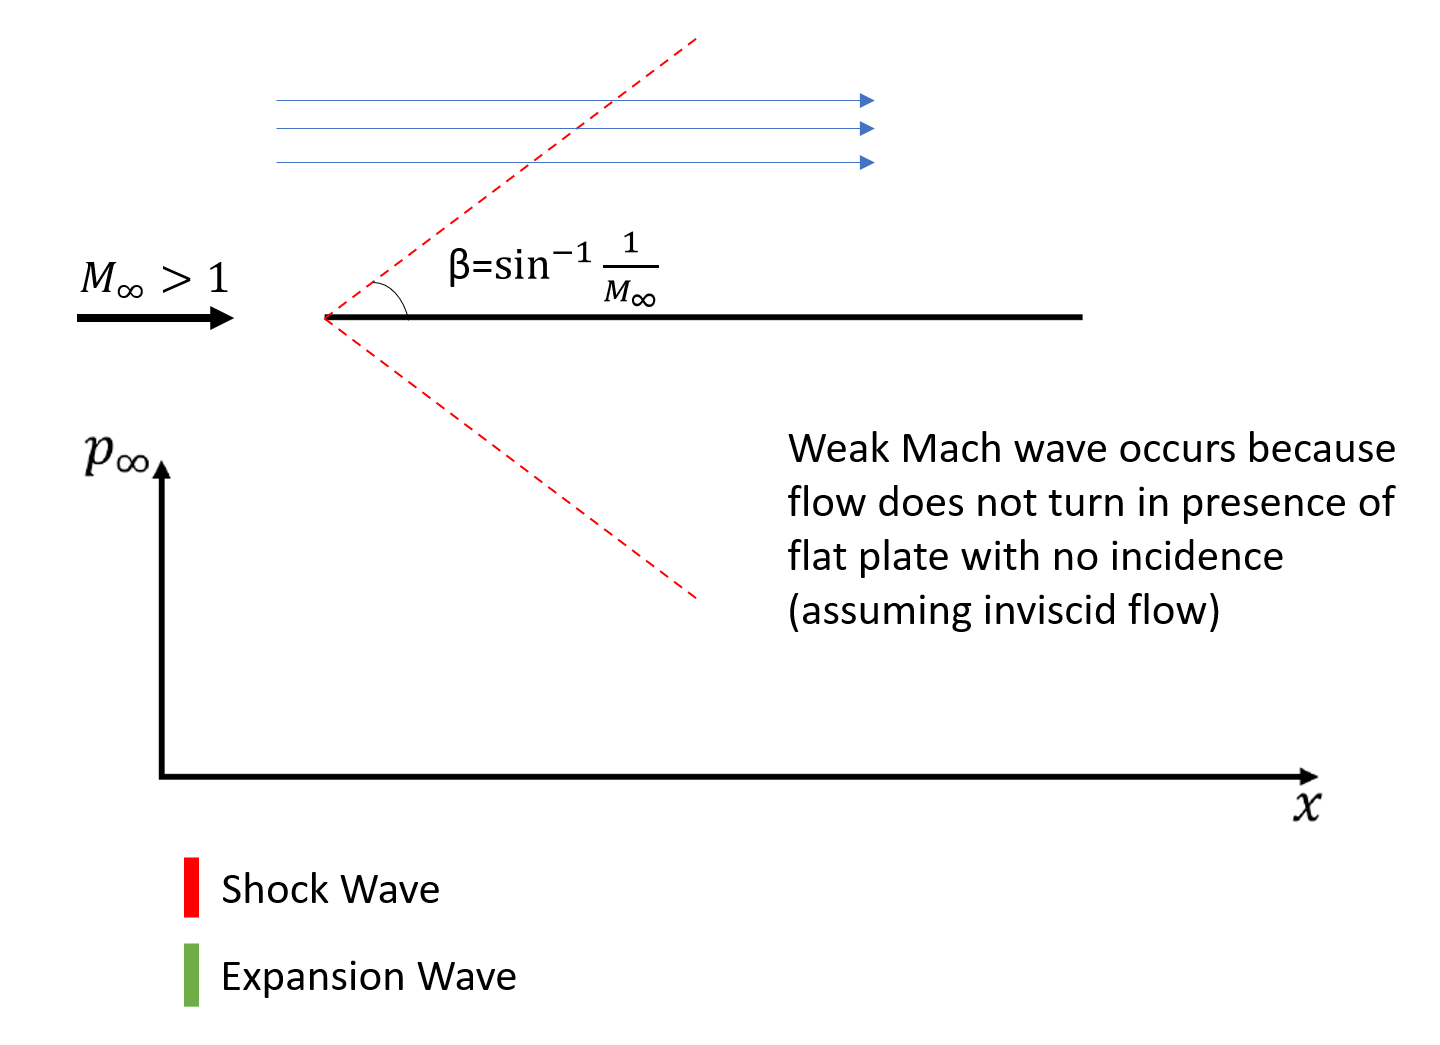
\includegraphics[scale=0.5]{../../images/problem_2/fig_11.png}
    \caption{Shock Diagram: Flat plate with no incidence}
    \label{flat_shock}
\end{figure}

\begin{figure}[h!]
    \centering
    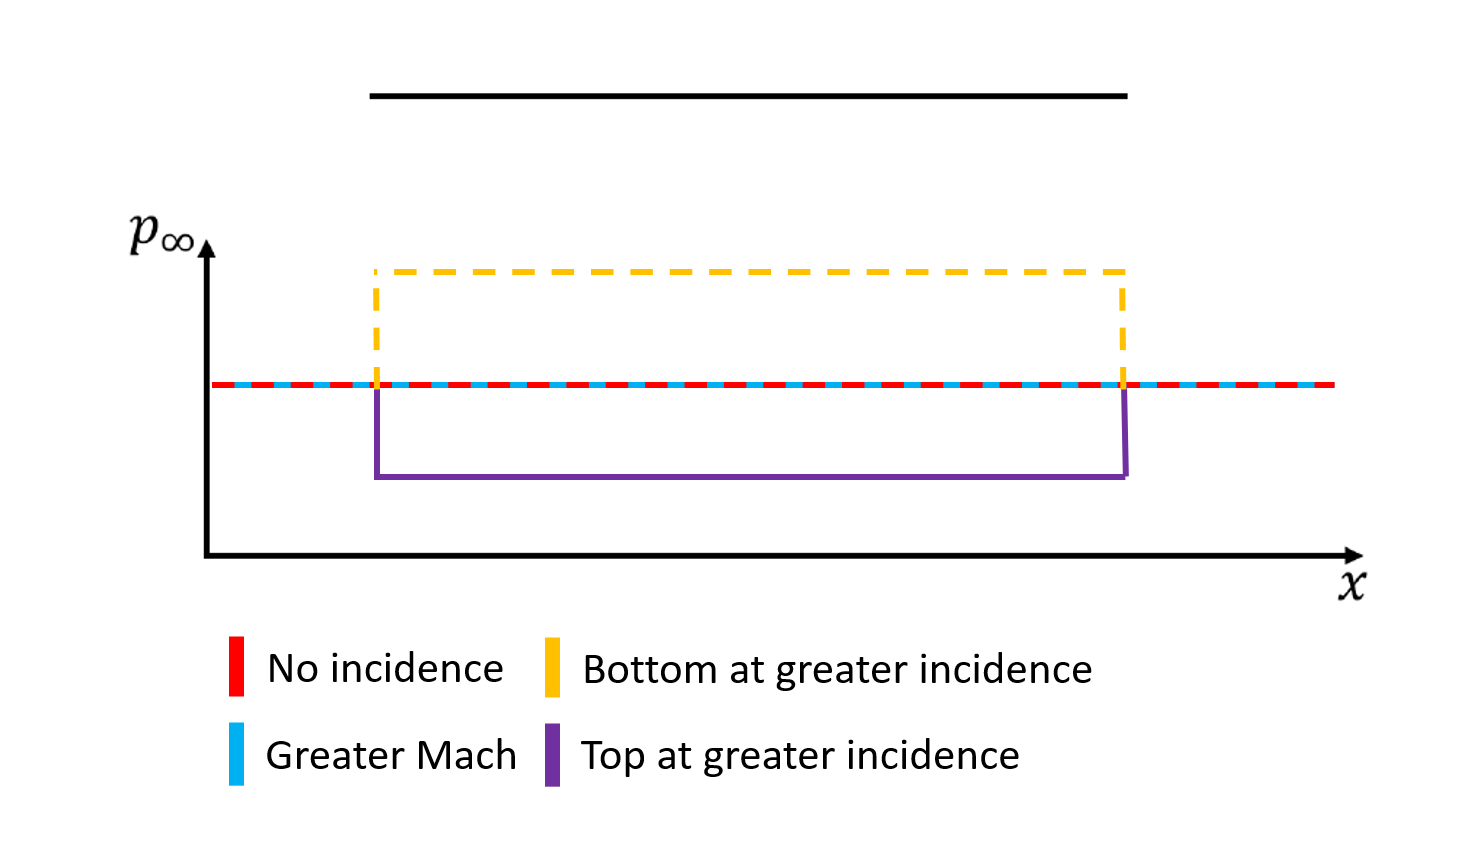
\includegraphics[scale=0.5]{../../images/problem_2/fig_12.png}
    \caption{Pressure Plot: Flat plate with no incidence}
    \label{flat_pressure}
\end{figure}

\begin{figure}[h!]
    \centering
    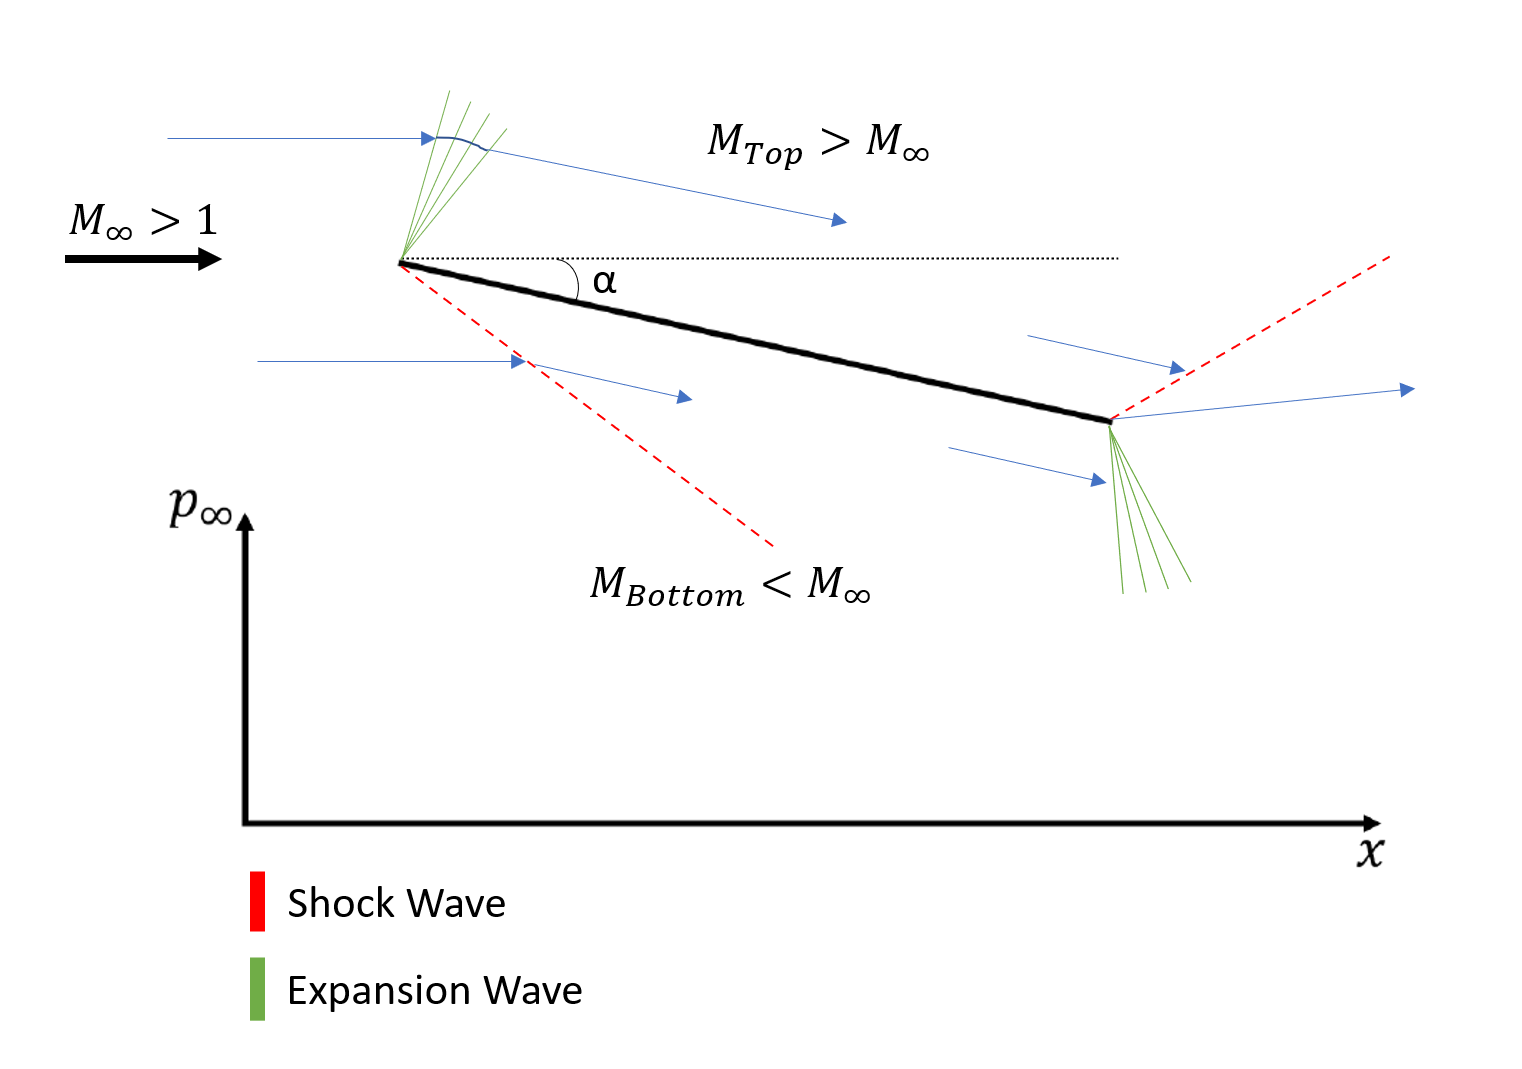
\includegraphics[scale=0.5]{../../images/problem_2/fig_21.png}
    \caption{Shock Diagram: Flat plate with incidence}
    \label{incidence_shock}
\end{figure}

\begin{figure}[h!]
    \centering
    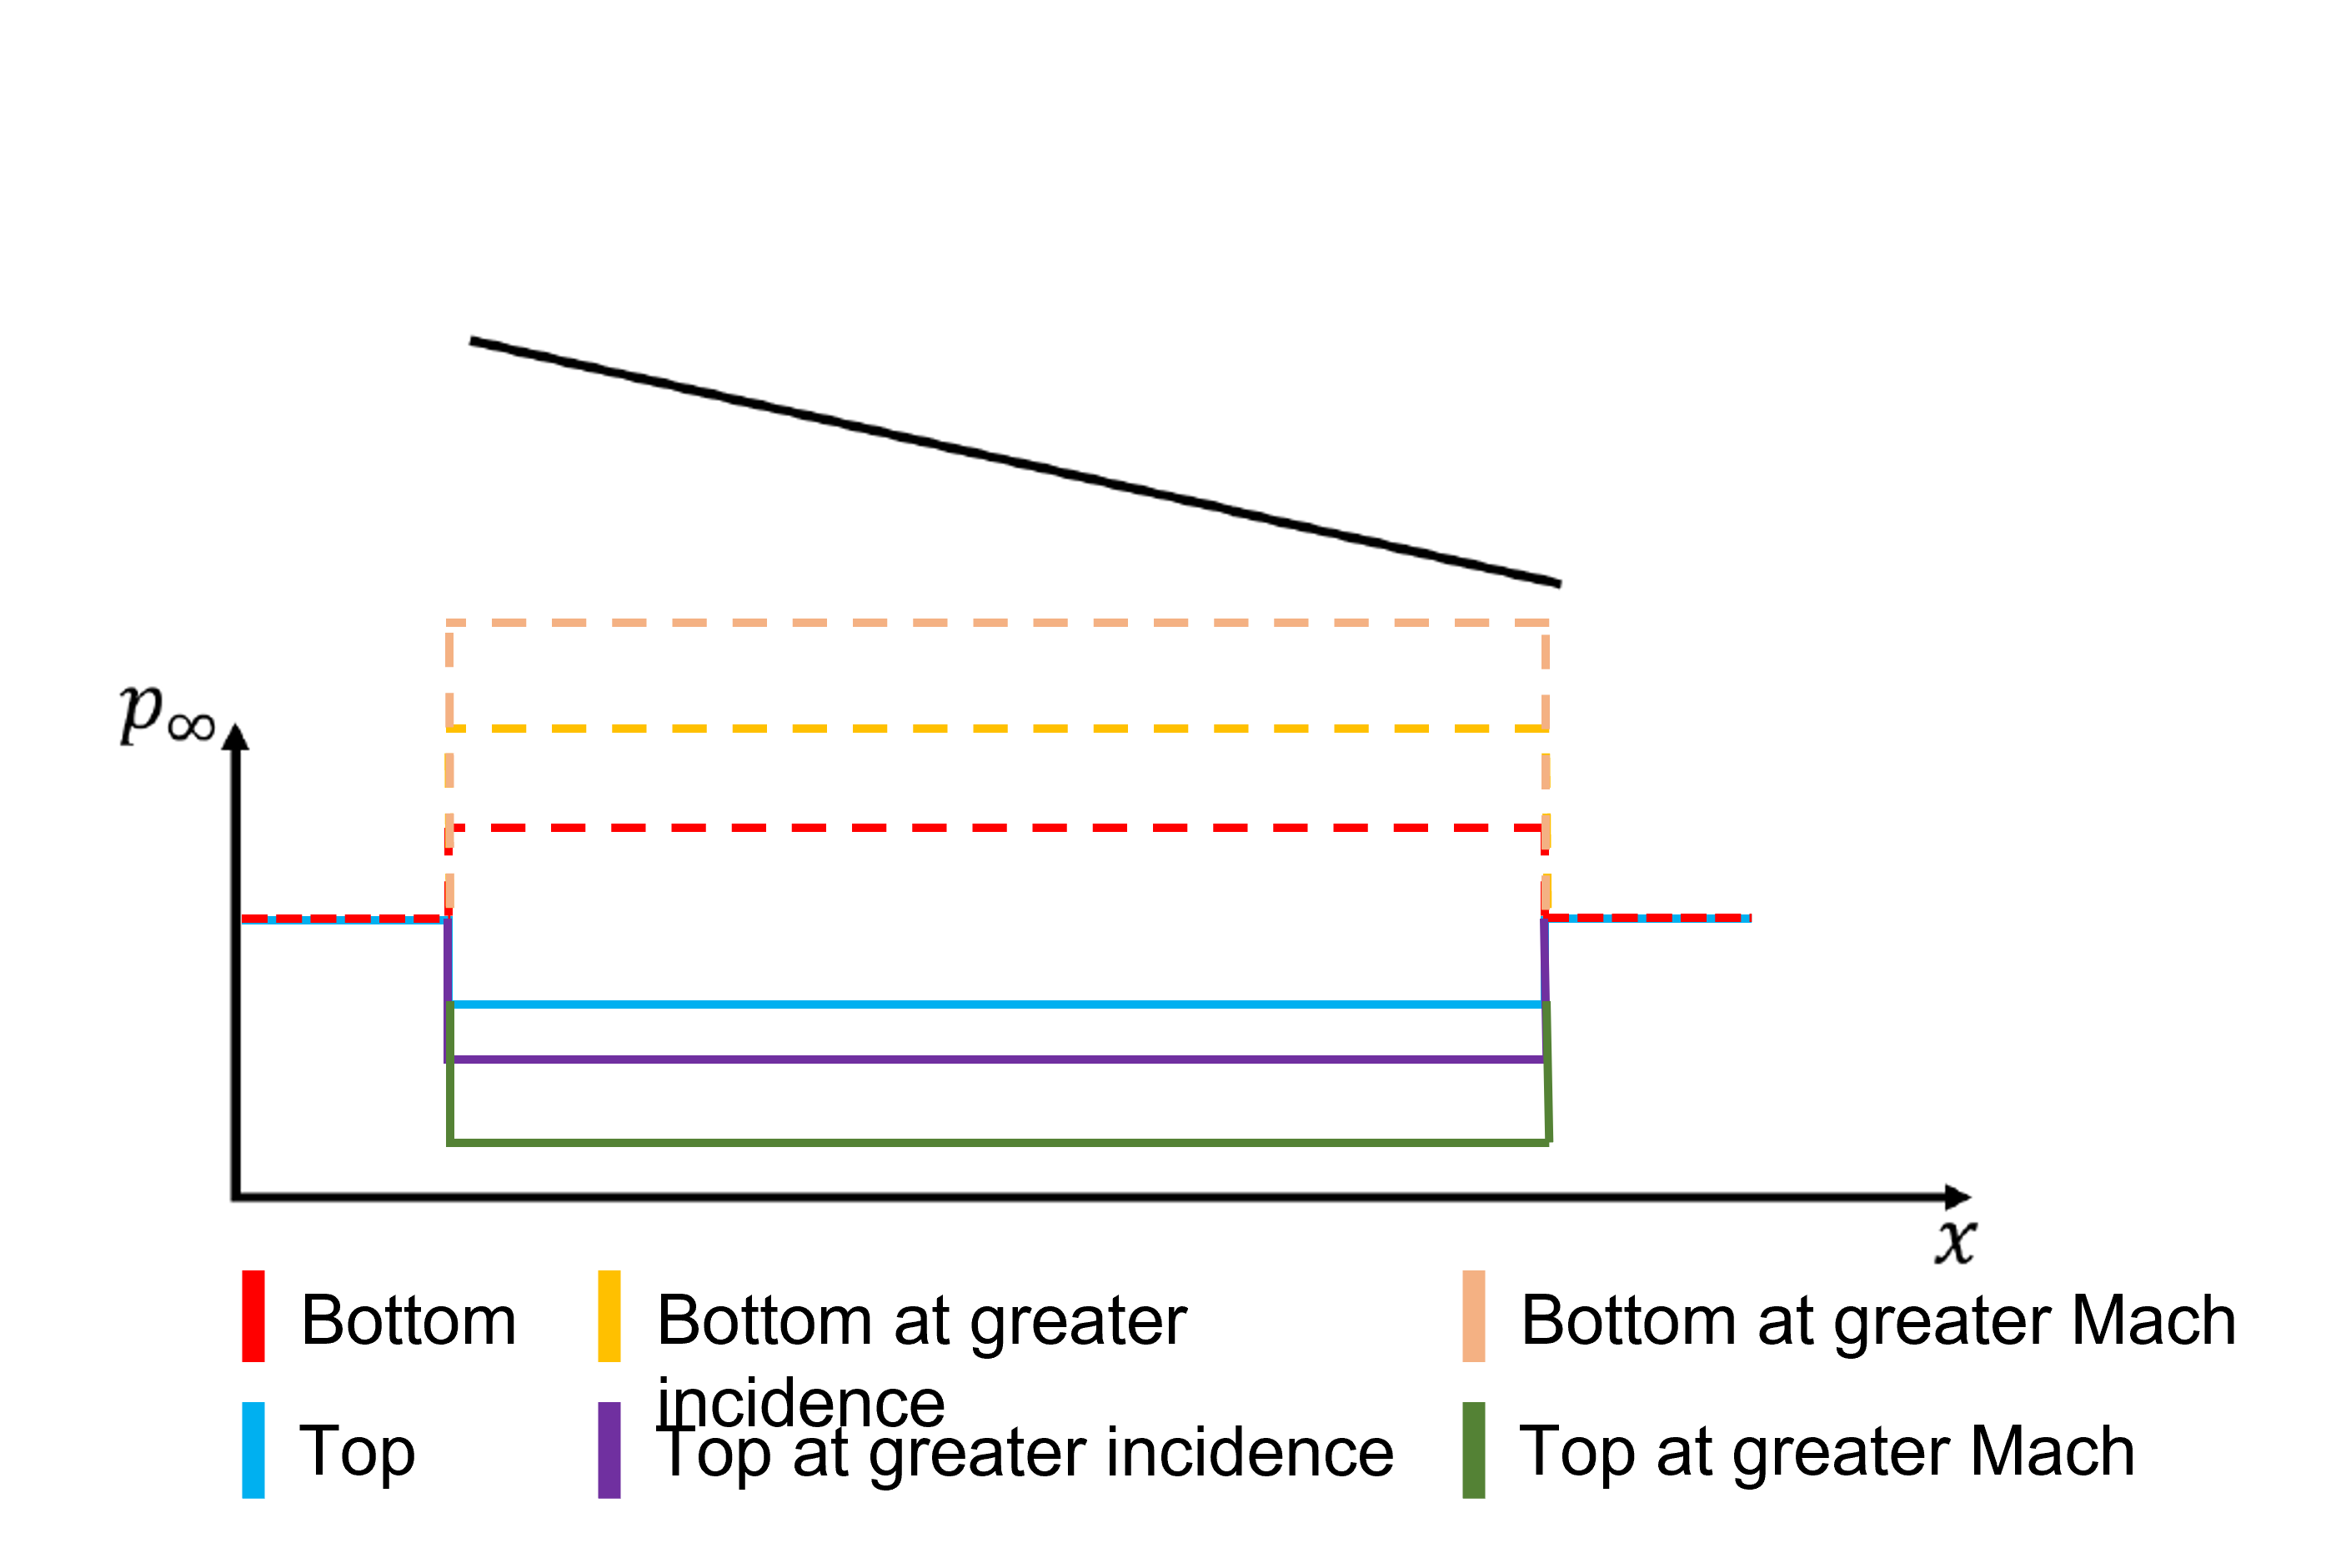
\includegraphics[scale=0.5]{../../images/problem_2/fig_22.png}
    \caption{Pressure Plot: Flat plate with incidence}
    \label{incidence_pressure}
\end{figure}

\begin{figure}[h!]
    \centering
    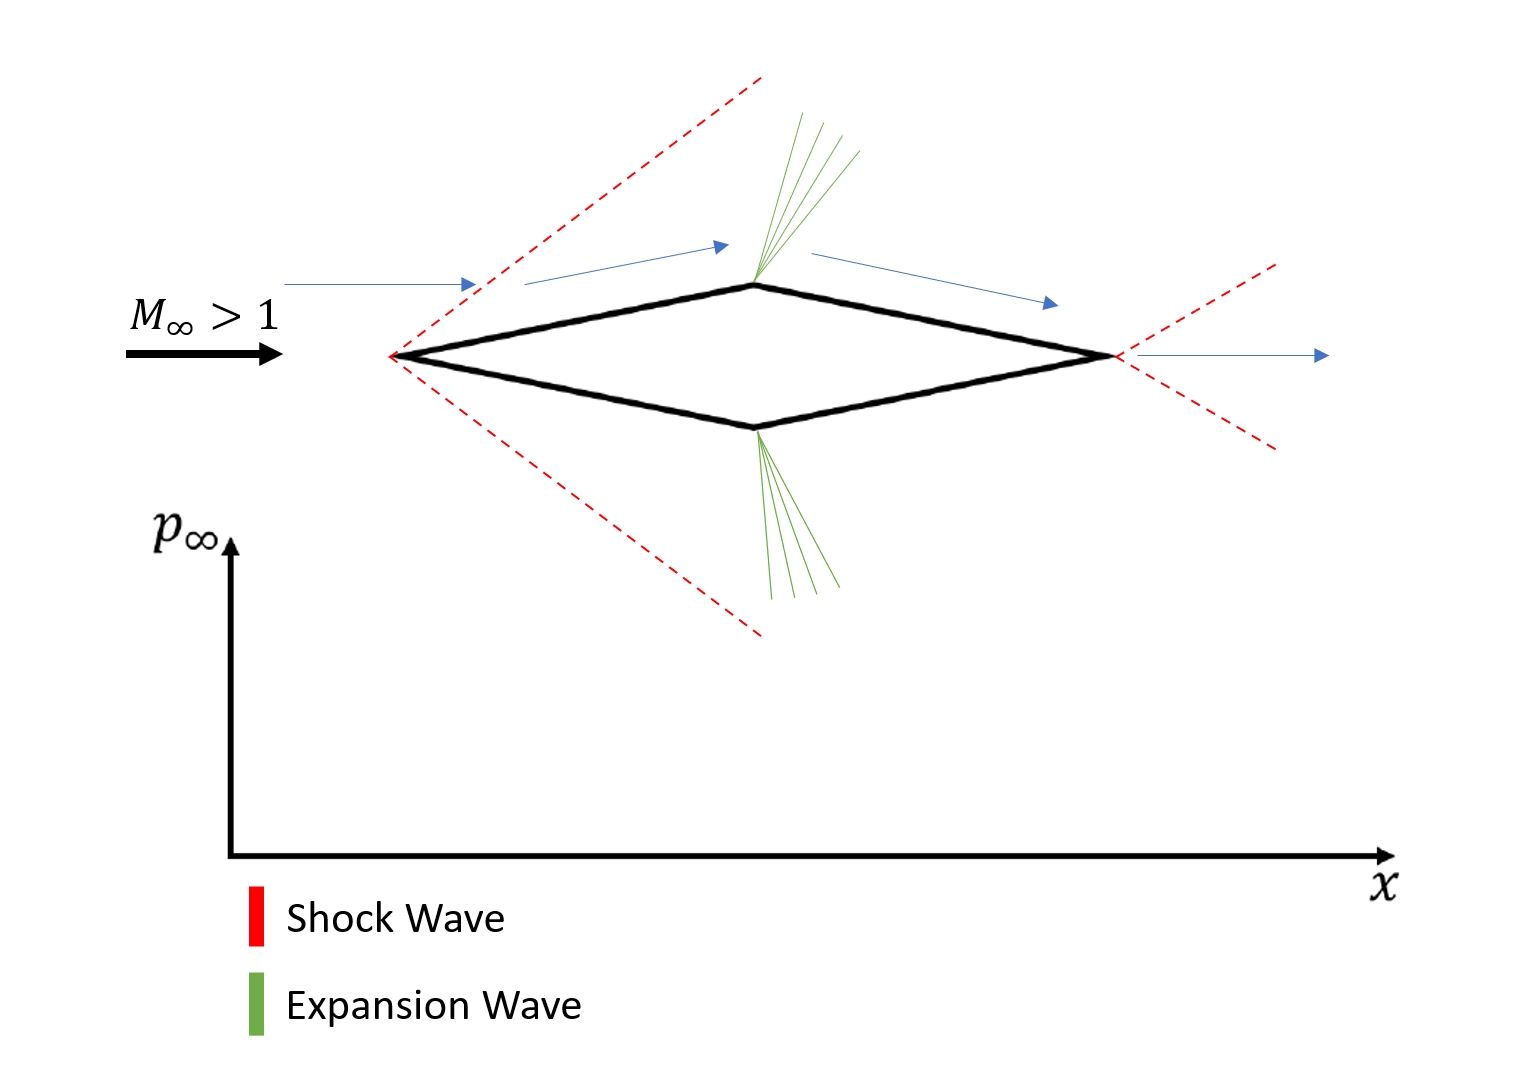
\includegraphics[scale=0.5]{../../images/problem_2/fig_31.png}
    \caption{Shock Diagram: Diamond wedge}
    \label{diamond_shock}
\end{figure}

\begin{figure}[h!]
    \centering
    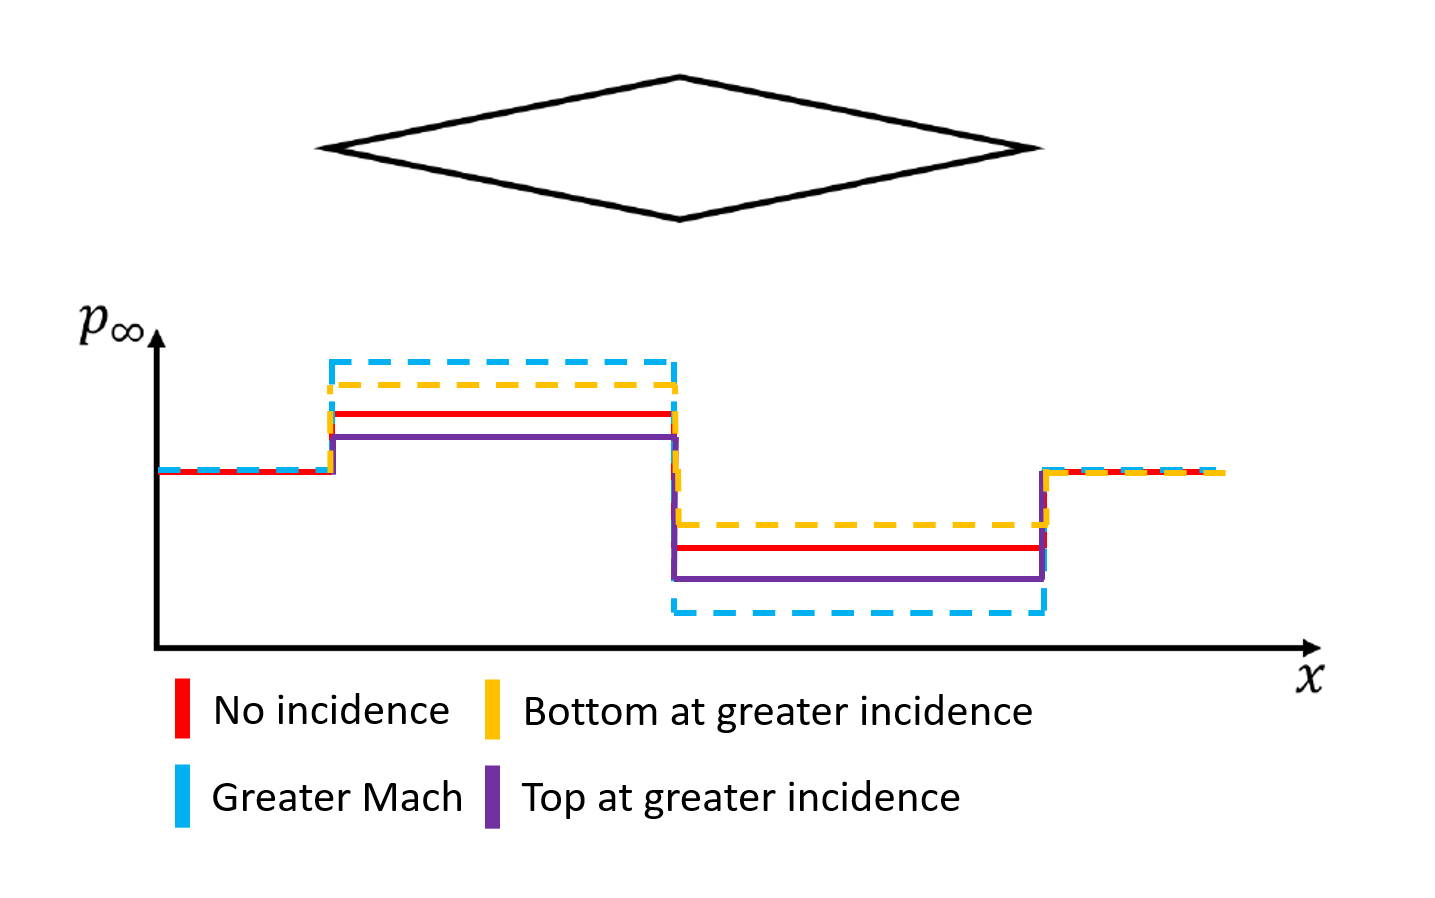
\includegraphics[scale=0.5]{../../images/problem_2/fig_32.png}
    \caption{Pressure Plot: Diamond wedge}
    \label{diamond_pressure}
\end{figure}

\begin{figure}[h!]
    \centering
    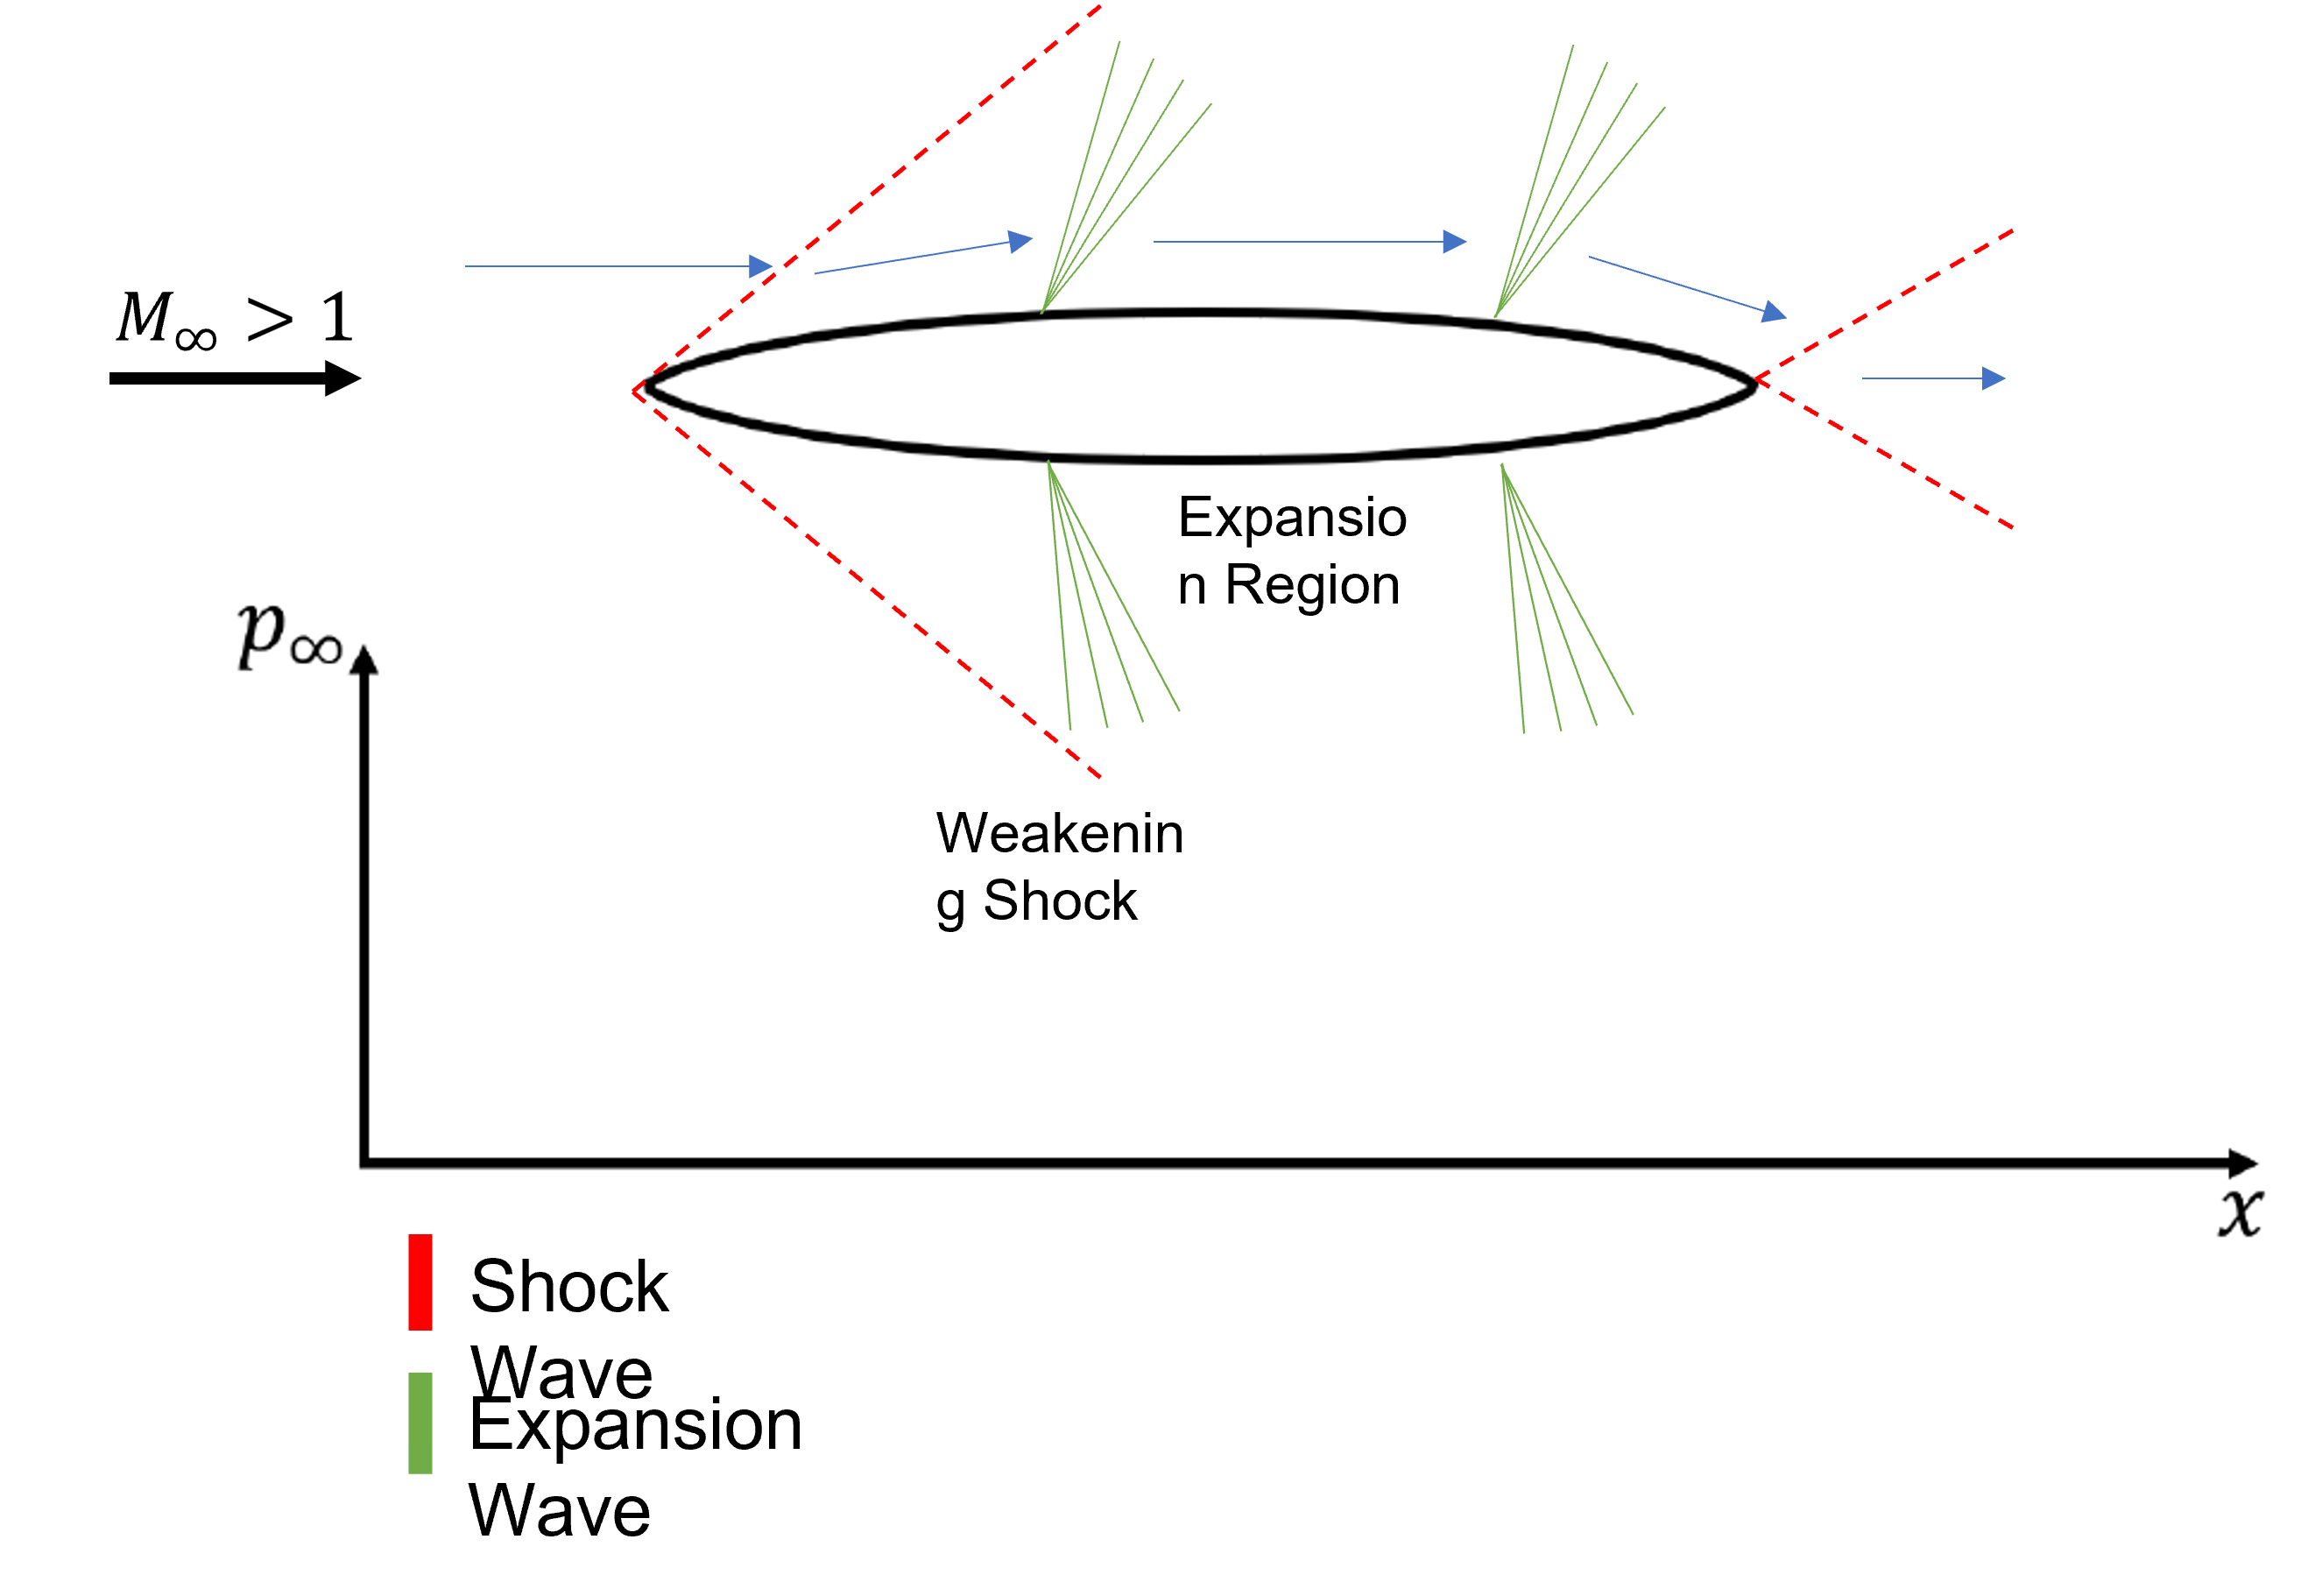
\includegraphics[scale=0.5]{../../images/problem_2/fig_41.png}
    \caption{Shock Diagram: Biconvex}
    \label{bi_shock}
\end{figure}

\begin{figure}[h!]
    \centering
    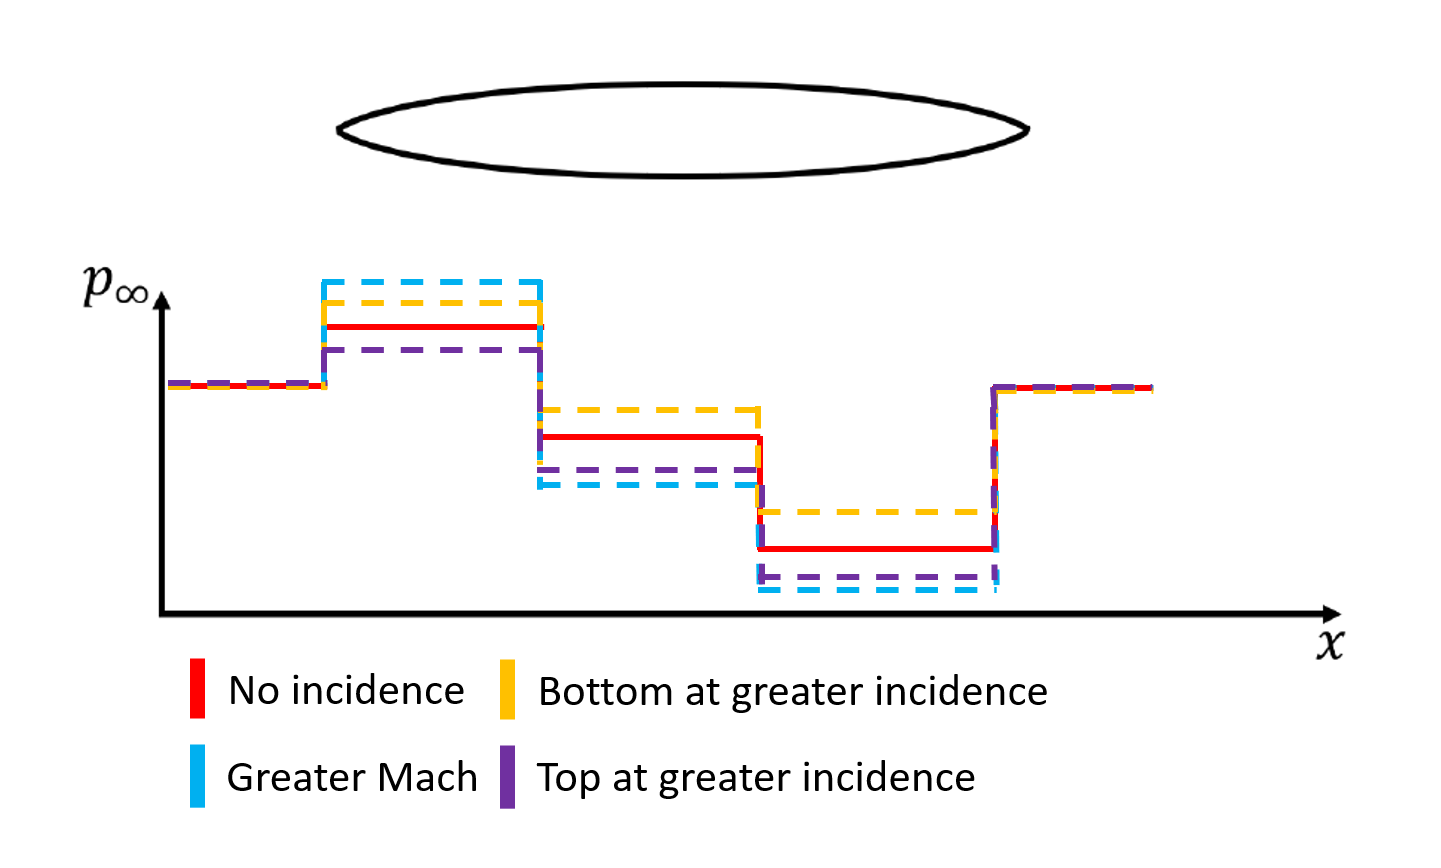
\includegraphics[scale=0.5]{../../images/problem_2/fig_42.png}
    \caption{Pressure Plot: Biconvex}
    \label{bi_pressure}
\end{figure}

\begin{figure}[h!]
    \centering
    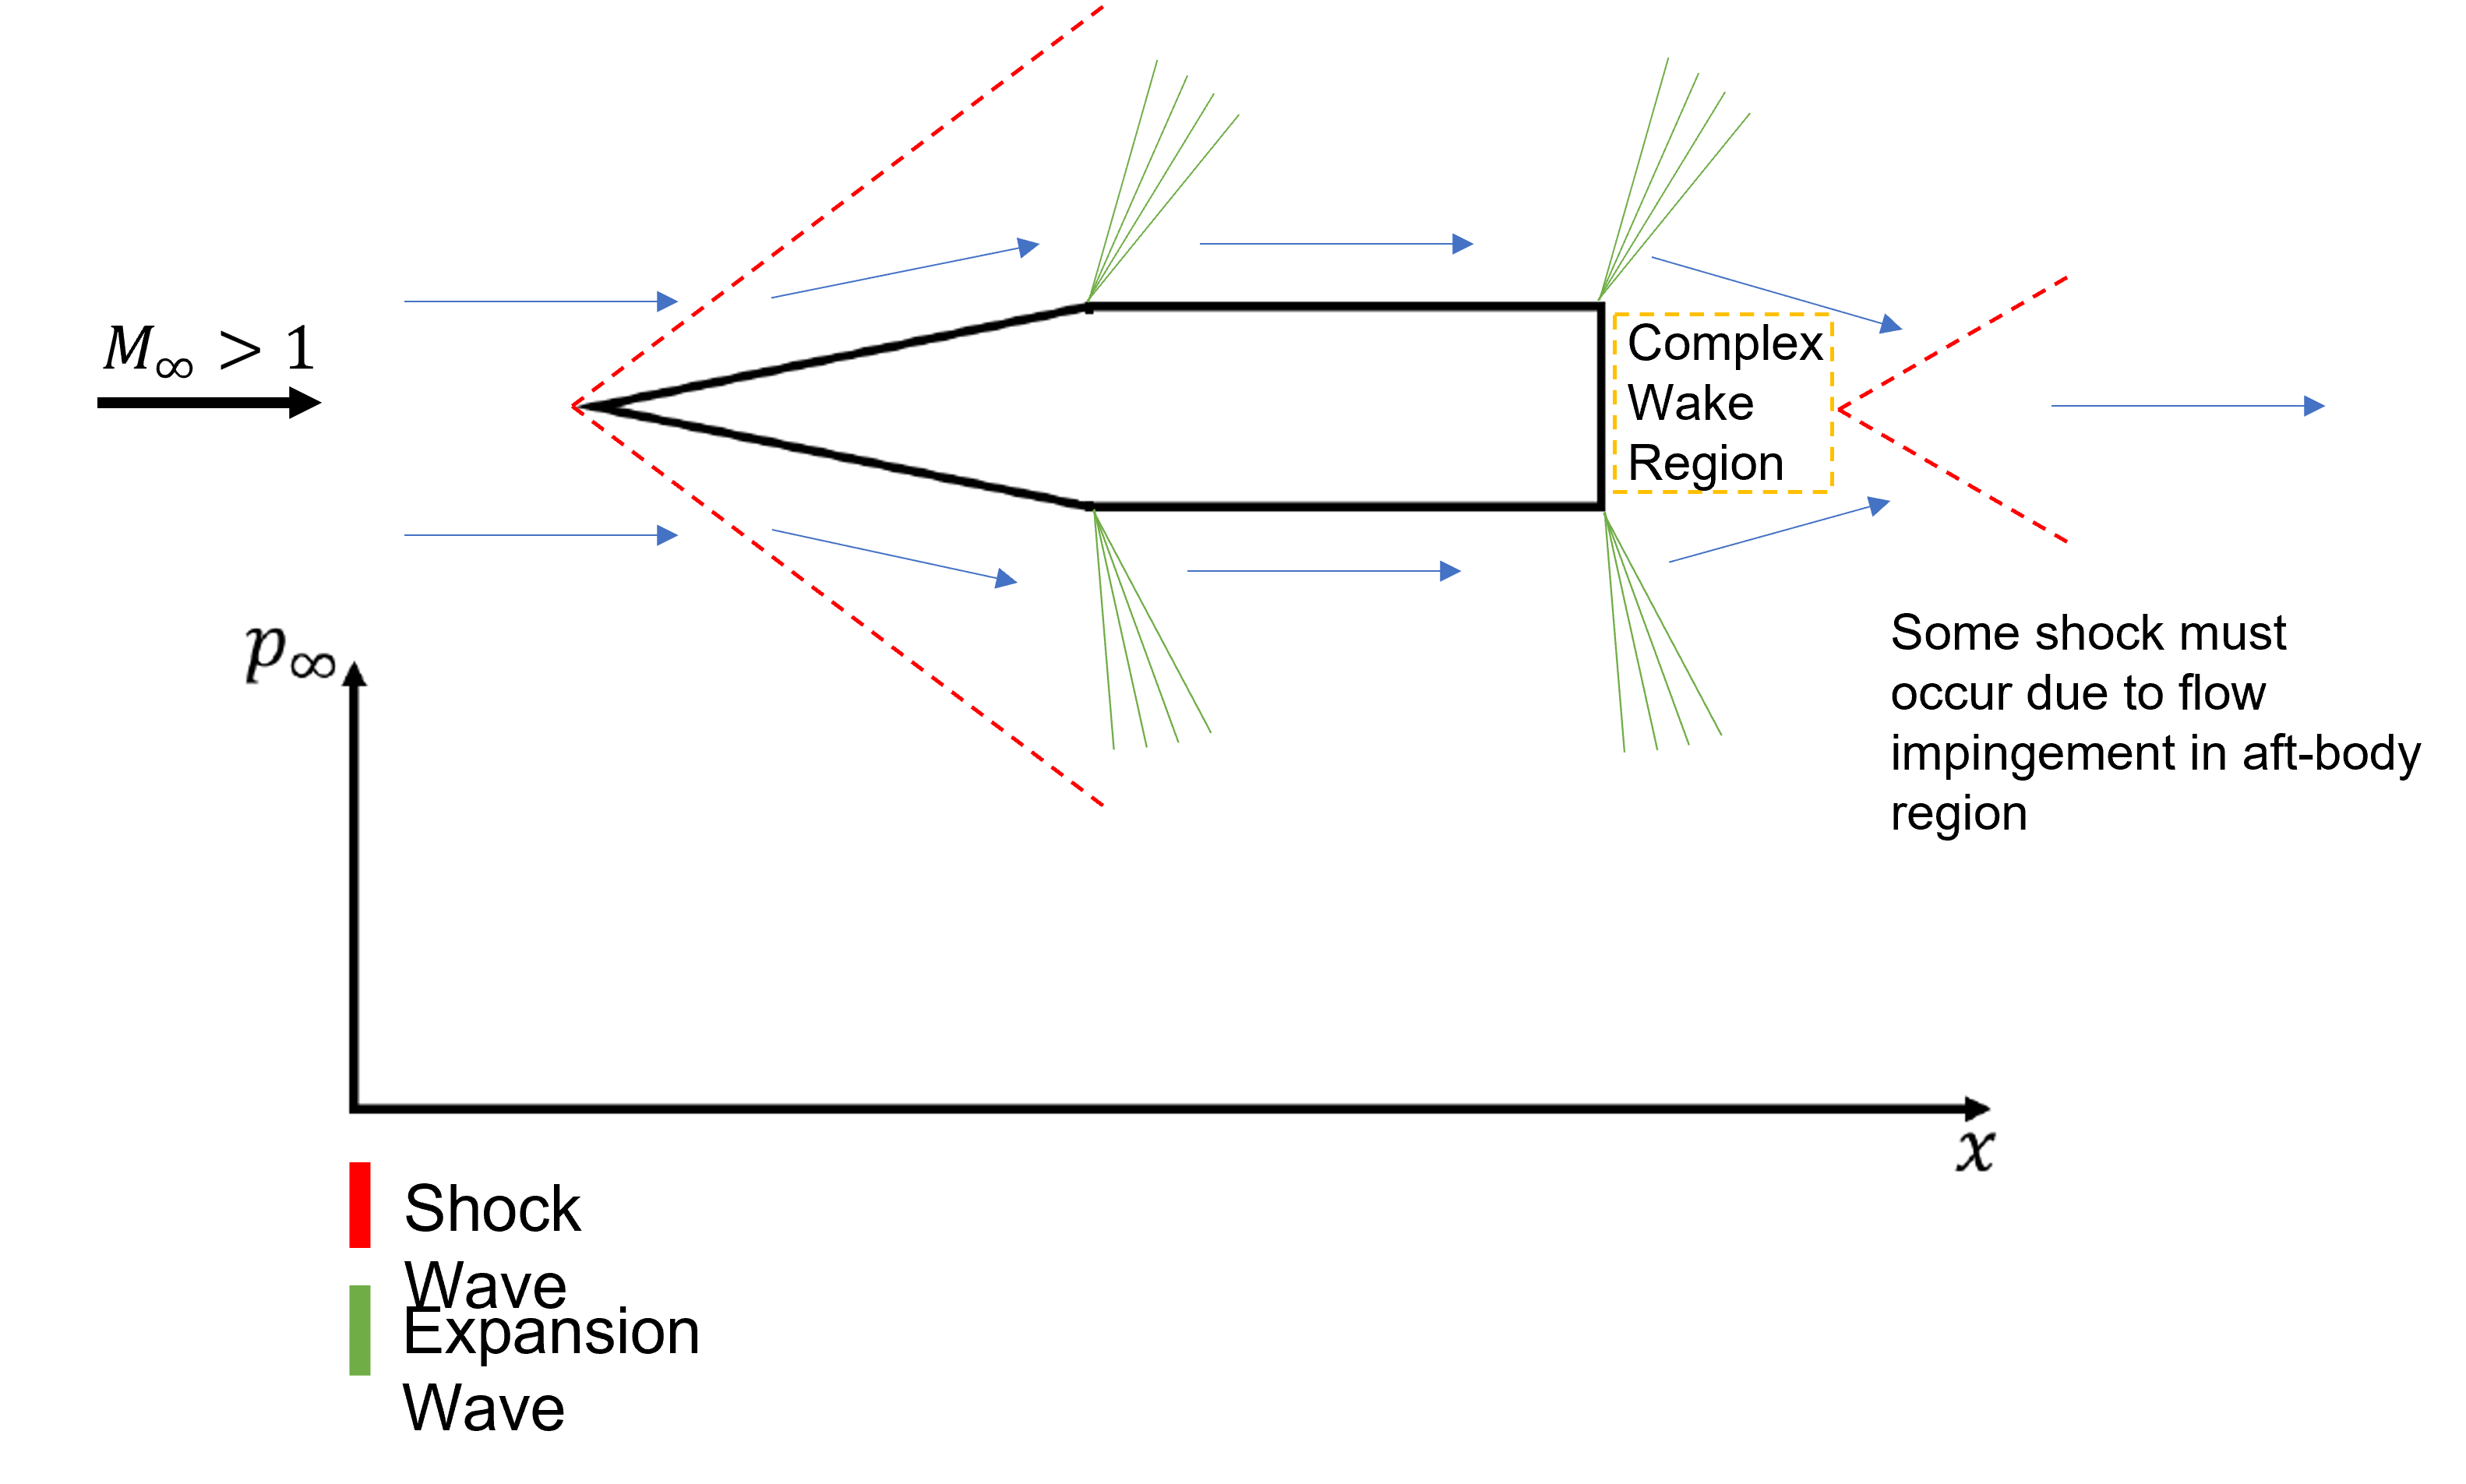
\includegraphics[scale=0.5]{../../images/problem_2/fig_51.png}
    \caption{Shock Diagram: Diamond block}
    \label{block_shock}
\end{figure}

\begin{figure}[h!]
    \centering
    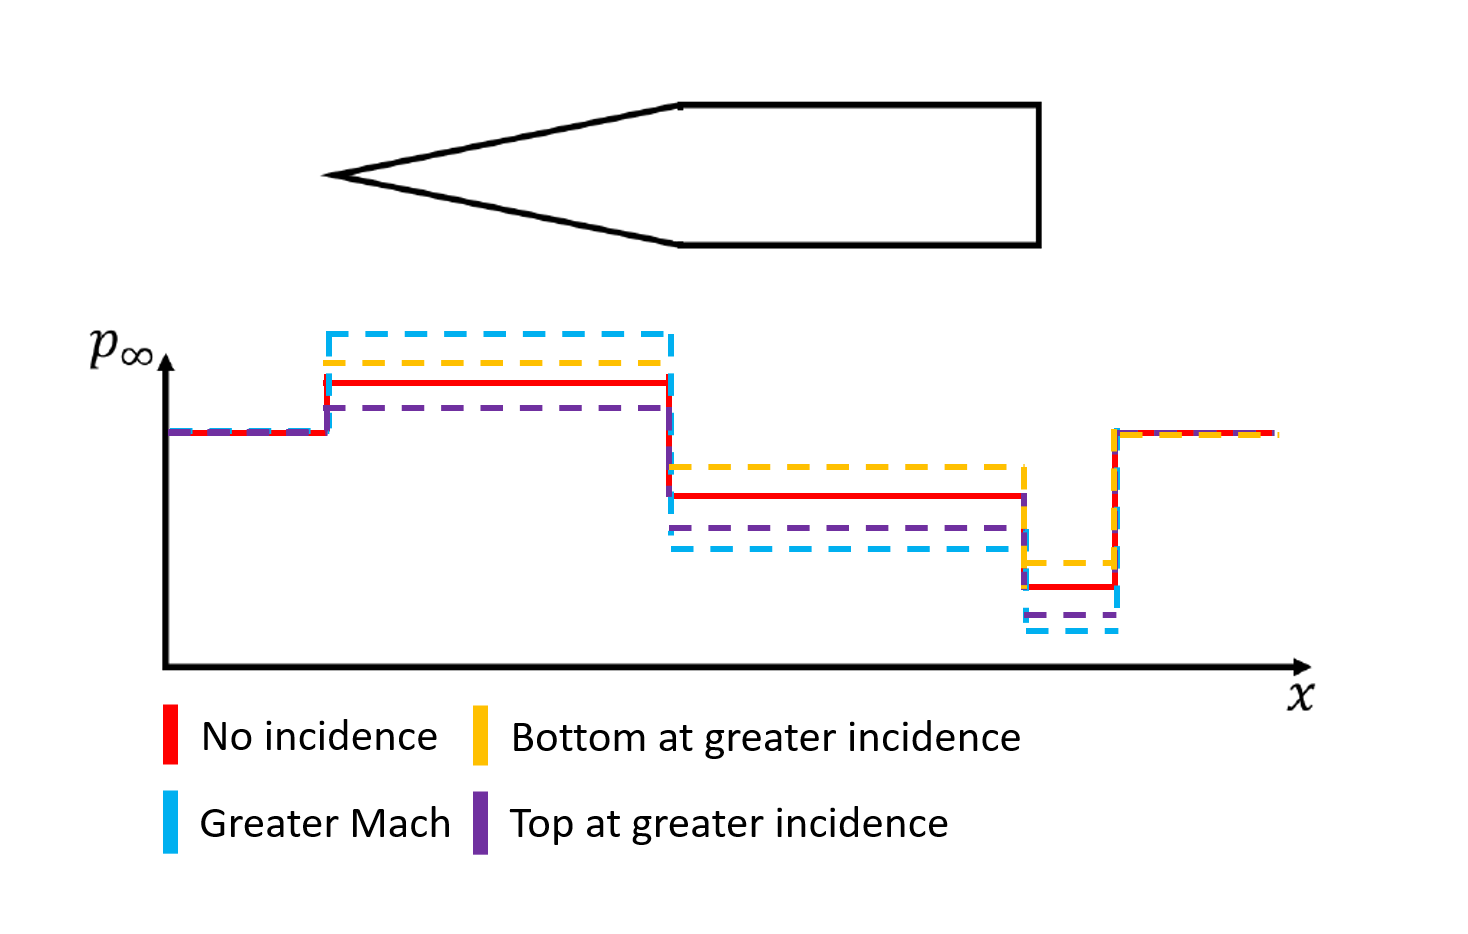
\includegraphics[scale=0.5]{../../images/problem_2/fig_52.png}
    \caption{Pressure Plot: Diamond block}
    \label{block_pressure}
\end{figure}

\end{document}